\documentclass[]{beamer}
\usepackage{beamerthemesplit}
\usepackage{graphics,epsfig}
\usepackage{pstricks}
\usepackage{graphicx}
\usepackage{hyperref}
\usepackage{subfigure}
\usepackage{listings}
\usepackage{multirow}
\usepackage{xspace}
\usepackage[absolute,overlay]{textpos}
\usepackage{tikz}
\usetikzlibrary{decorations}
\usetikzlibrary{decorations.pathmorphing}
\usetikzlibrary{shapes,arrows}
\setlength{\TPHorizModule}{1cm}
\setlength{\TPVertModule}{1cm}


\mode<presentation>
{ \usetheme{Boadilla}
  \setbeamercovered{transparent}
  \setbeamertemplate{items}[circle]
  \setbeamertemplate{theorems}[numbered]
  \setbeamertemplate{footline}[frame number]
}
 
%\useinnertheme[shadow=true]{rounded}
\useoutertheme{shadow}
\usecolortheme{whale}

\newcommand\blfootnote[1]{
  \begingroup
  \renewcommand\thefootnote{}\footnote{#1}
  \addtocounter{footnote}{-1}
  \endgroup
}

\mode
<all>

\title{C Programming}
\author{Wan-Lei Zhao}

\makeatletter

\begin{document}
\begin{frame}
   \begin{center}
    \vspace{24pt}
    \Huge\textbf{C Programming}\blfootnote{Email: wlzhao@xmu.edu.cn, copyrights are fully reserved by the author.}\\
     %\Huge{Lecture 9: Operations on File}
     \begin{figure}
     	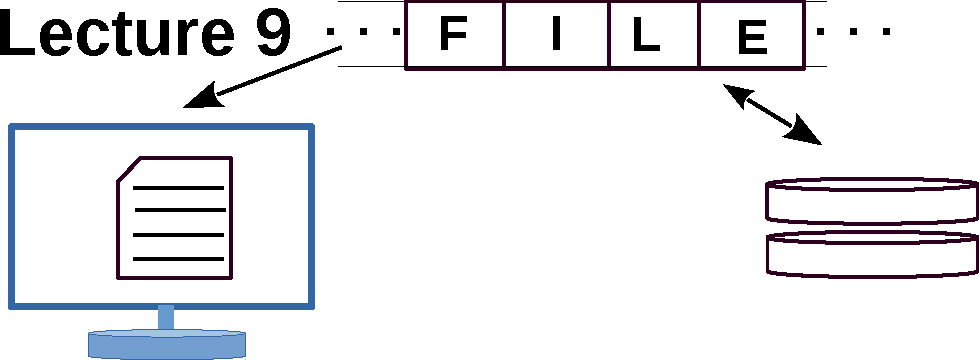
\includegraphics[width=0.6\linewidth]{figs/file_symb.pdf}
     \end{figure}
    \vspace{36pt}
  \end{center}
  \begin{align*}
   \vspace{18pt}
      \large{\mbox{Lecturer:}~Dr.~\mbox{Wan-Lei~~Zhao}} \\
      \large{Spring~~Semester~~2022} \\
   \vspace{30pt}
  \end{align*}
\end{frame}

\definecolor{cornblue}{HTML}{6495ED}
\definecolor{navyblue}{HTML}{000080}
\definecolor{midnblue}{HTML}{191970}
\definecolor{lghtblue}{HTML}{B0C4DE}
\setbeamercolor{background}{fg=black, bg=lghtblue}
\setbeamercolor{palette primary}{fg=white, bg=lghtblue}
\setbeamercolor{palette secondary}{fg=black, bg=cornblue}
\setbeamercolor{palette tertiary}{fg=black, bg=lghtblue}
\setbeamercolor{palette quaternary}{fg=black, bg=lghtblue}
\setbeamercolor{frametitle}{fg=black, bg=white}
\definecolor{ballblue}{rgb}{0.13, 0.67, 0.8}
\definecolor{cornflowerblue}{rgb}{0.39,0.58,0.93}
\definecolor{babyblueeyes}{rgb}{0.63, 0.79, 0.95}

\setbeamertemplate{footline}
{
  \leavevmode%
  \hbox{%
  \begin{beamercolorbox}[wd=.275\paperwidth,ht=2.25ex,dp=1ex,center]{author in head/foot}%
    \usebeamerfont{author in head/foot}\insertshortauthor
  \end{beamercolorbox}%
  \begin{beamercolorbox}[wd=.44\paperwidth,ht=2.25ex,dp=1ex,center]{title in head/foot}%
    \usebeamerfont{title in head/foot}\insertshorttitle\hspace*{3em}
    \hspace*{1ex}
  \end{beamercolorbox}%
  \begin{beamercolorbox}[wd=.285\paperwidth,ht=2.25ex,dp=1ex,center]{date/foot}%
    \usebeamerfont{title in head/foot}\hspace*{2em}
    \insertframenumber{} / \inserttotalframenumber\hspace*{1ex}
  \end{beamercolorbox}}%
  \vskip0pt
}



% preset-listing options
\lstset{
  backgroundcolor=\color{white},   
  basicstyle=\footnotesize,    
  language=c,
  breakatwhitespace=false,         
  breaklines=true,                 % sets automatic line breaking
  captionpos=b,                    % sets the caption-position to bottom
  commentstyle=\color{ballblue},    % comment style
  extendedchars=true,              
  frame=single,                    % adds a frame around the code     
  keywordstyle=\color{blue},       % keyword style
  numbers=left,                    
  numbersep=5pt,                   
  numberstyle=\tiny\color{blue}, 
  rulecolor=\color{babyblueeyes},
  stepnumber=1,              
  stringstyle=\color{black},     % string literal style
  tabsize=4,                       % sets default tabsize to 4 spaces
  title=\lstname                   
}


\section{Overview about Computer Storage}
\label{sec:overview}
\begin{frame}<beamer>
    \frametitle{Outline}
    \tableofcontents[currentsection]
\end{frame}

\begin{frame}{Overview}
\begin{itemize}
	\item {When we doing programming}
	\item {Or run our code}
	\item {Two main components of a computer we work with}
	\begin{enumerate}
		\item {CPU: where our codes are executed}
		\item {Memory: where our codes are \textcolor{red}{temporarily} kept}
	\end{enumerate}
	\item {When computer is switched off}
	\item {Everything resides in memory disappear}
	\item {External storage is where we can keep things \textcolor{red}{permanently}}
\end{itemize}
\end{frame}

\begin{frame}{Storage Device (1)}
\begin{figure}
	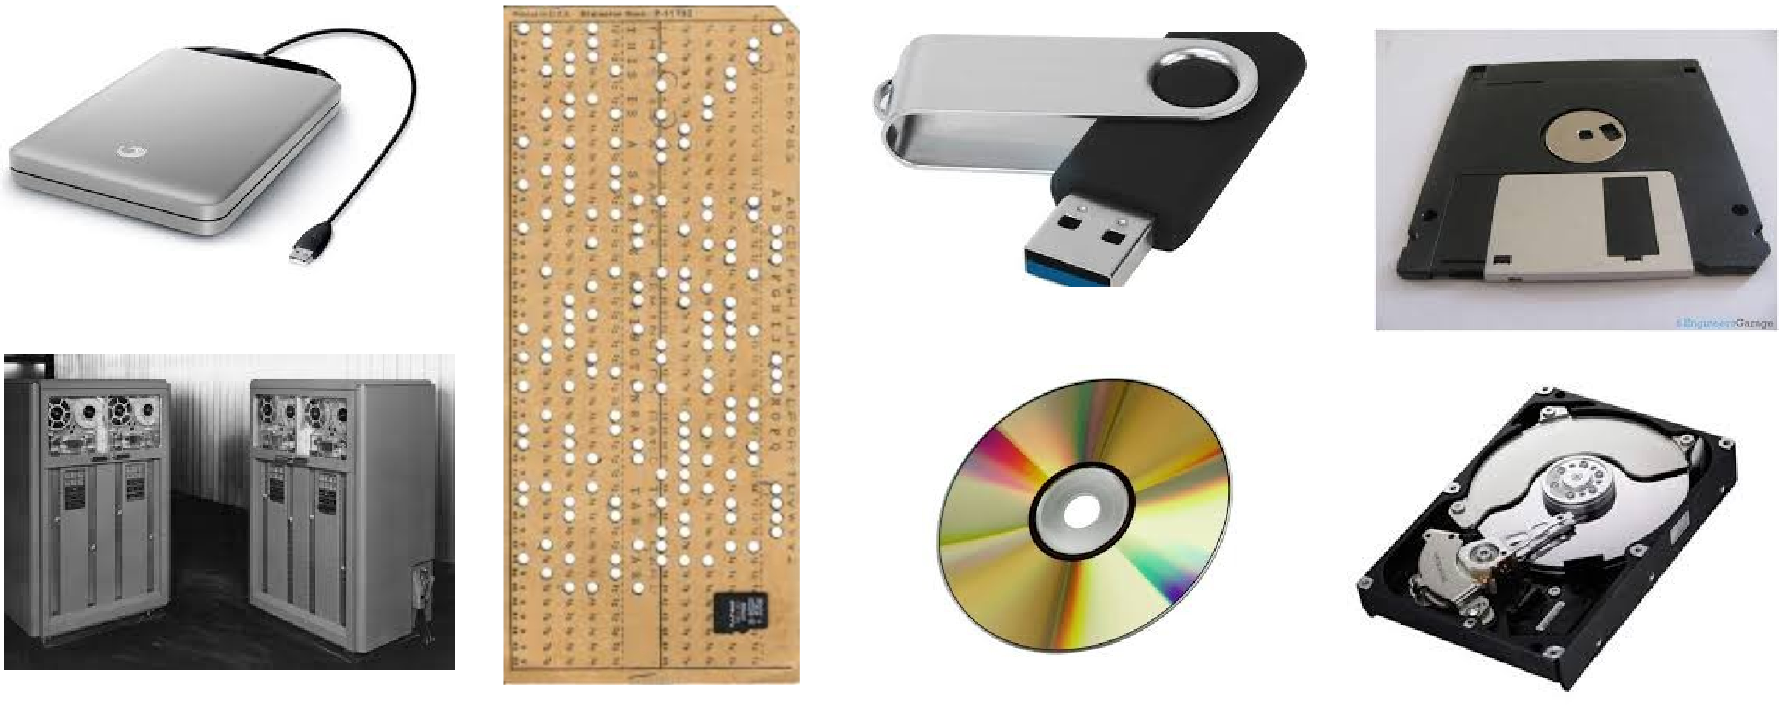
\includegraphics[width=0.9\linewidth]{figs/storages.pdf}
\end{figure}
\begin{itemize}
	\item {There are all kinds of storage devices in the history of computer}
	\item {Currently, hard disc (it is hard), DVD and USB are popular}
	\item {Things are kept there in the unit of \textbf{file}}
\end{itemize}
\end{frame}

\begin{frame}{Storage Device (2)}
\begin{itemize}
	\item {There are several basic thing should be kept for a file}
	\begin{enumerate}
		\item {File name}
		\item {File size}
		\item {Location in the disc: which cylinder, which track and which sector?}
		\item {Time the file created, updated and the last time file is read}
		\item {Anything else??}
	\end{enumerate}
\end{itemize}
\begin{figure}
	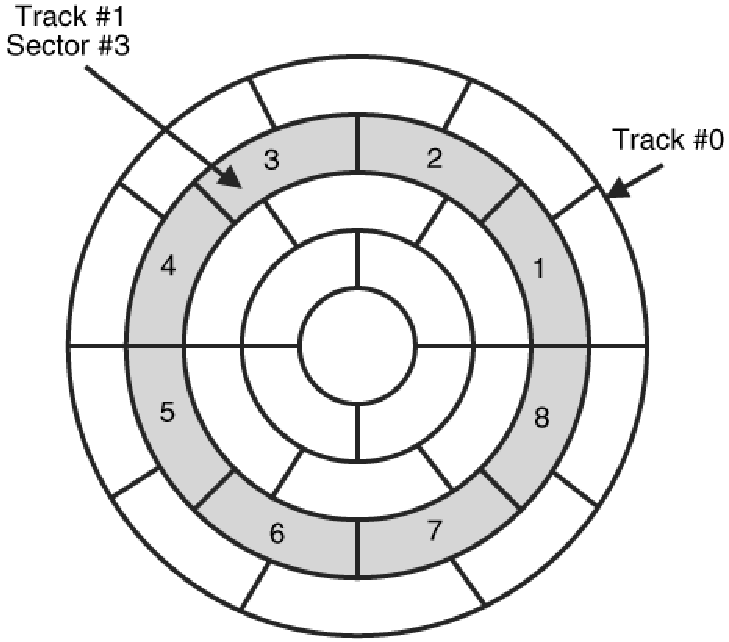
\includegraphics[width=0.35\linewidth]{figs/disc.pdf}
\end{figure}
\end{frame}

\begin{frame}{Storage Device (3)}
\begin{itemize}
	\item {There are several basic thing should be kept for a file}
	\begin{enumerate}
		\item {File name}
		\item {File size}
		\item {Location in the disc: which cylinder, which track and which sector?}
		\item {Time the file created, updated and the last time file is read}
		\item {Logic location: \textcolor{red}{full path} of the file: ``c:/docs/codes/hi.c''}
	\end{enumerate}
	\item {We use a \textcolor{blue}{struct} type to define such kind of information}
\end{itemize}
\begin{figure}
	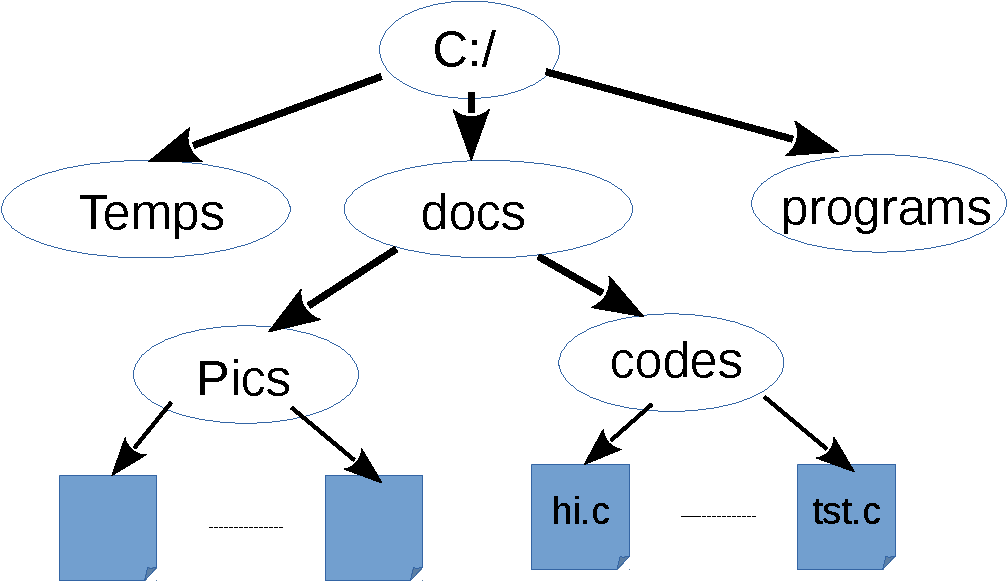
\includegraphics[width=0.5\linewidth]{figs/ftree.pdf}
\end{figure}
\end{frame}

\section{Operation on Files}
\label{sec:file}
\begin{frame}<beamer>
    \frametitle{Outline}
    \tableofcontents[currentsection]
\end{frame}

\begin{frame}{Flow of File Operation in C}
\begin{figure}
	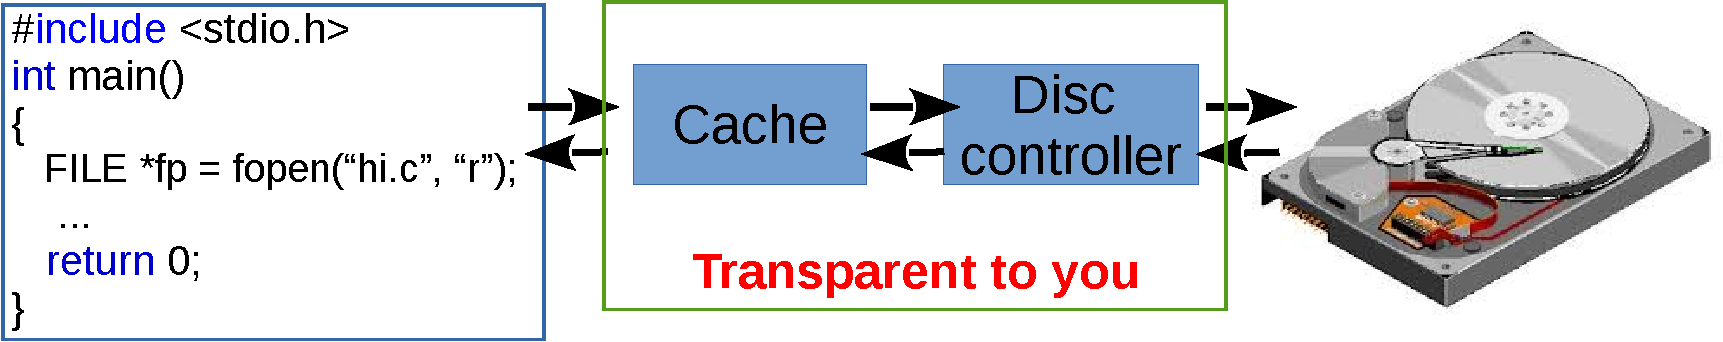
\includegraphics[width=0.95\linewidth]{figs/flowfio.pdf}
\end{figure}
\begin{itemize}
	\item {When file is open (for write/read)}
	\item {A cache is created in the memory}
	\item {Data are put to cache from either side first}
	\item {Transfer to another side later}
\end{itemize}
\end{frame}

\begin{frame}[fragile]{Read File in C (1)}
\vspace{-0.15in}
\begin{itemize}
	\item {A file name (with path) should be given}
	\begin{itemize}
		\item {full path: ``c:/docs/codes/hi.c''}
		\item {relative path: ``../codes/hi.c''}
	\end{itemize}
	\item {Tell the system, you are going to read ("r") the file}
\end{itemize}
\begin{lstlisting}[xleftmargin=0.06\linewidth, linewidth=0.85\linewidth]
#include <stdio.h>
int main()
{
  const char *fn = "c:/docs/codes/hi.txt";
  int a = 0, b = 0;
  FILE *fp = fopen(fn, "r");
  if(fp == NULL)//in case that open file failed
  { //required all the time
     printf("Open file %d\n failed", fn);
     return 0;
  }
  fscanf(fp, "%d%d", &a, &b);
  fclose(fp); //This is required all the time
  printf("%d %d\n", a, b);
  return 0;
}
\end{lstlisting}
\end{frame}


\begin{frame}[fragile]{FILE struct type}
\vspace{-0.15in}
\begin{columns}
\begin{column}{0.47\linewidth}
\begin{lstlisting}
#include <stdio.h>
int main()
{
  FILE *fp = fopen(fn, "r");
}
\end{lstlisting}
\end{column}
\begin{column}{0.49\linewidth}
\begin{lstlisting}[xleftmargin=0.1\linewidth, linewidth=0.90\linewidth]
typedef struct 
{
 short level;
 short token;
 short bsize;
 char fd;
 unsigned flags;
 unsigned char hold;
 unsigned char *buffer;
 unsigned char * curp;
 unsigned istemp; 
}FILE;
\end{lstlisting}
\end{column}
\end{columns}
\vspace{-0.2in}
\begin{itemize}
	\item {``FILE'' is a \textcolor{blue}{struct} designed for file operation}
	\item {It is defined in header ``$<$stdio.h$>$''}
\end{itemize}
\end{frame}


\begin{frame}[fragile]{Read File in C (2): the flow}
\tikzstyle{decision} = [diamond, draw, fill=yellow!20, 
    text width=6.5em, text badly centered, node distance=2cm, inner sep=0pt]
\tikzstyle{block} = [rectangle, draw, fill=blue!20, 
    text width=12em, text centered, rounded corners, minimum height=3em]
\tikzstyle{line} = [draw, -latex']
\tikzstyle{arrow} = [thick,->,>=stealth]
\tikzstyle{cloud} = [draw, ellipse,fill=red!20, node distance=2cm,
    minimum height=2em]
\begin{center}

\begin{tikzpicture}[node distance = 2.5cm, auto]
    % Place nodes
    \node [decision] (isopen) {if(fp != NULL)};
    \node [cloud, above of=isopen] (open) {FILE *fp = fopen("path", "r")};
    \node [block, below of=isopen, node distance=2.5cm] (read) {fscanf(fp, "\%s", oneline)};
    \node [cloud, below of=read, node distance=2cm] (close) {fclose(fp)};

    % Draw edges
    \path [line] (open) -- (isopen);
    %-- ++(3.0cm,0) |- node[anchor=west]
    \draw [arrow](isopen) -- ++(3.0cm,0) |- node[anchor=west]{no}(close);
    %\path [arrow] (isopen) -- node[near end]{no} (close);
    \path [line] (isopen) -- node [near end]{yes} (read);
    \path [line] (read) -- (close);
\end{tikzpicture}

\end{center}
\end{frame}

\begin{frame}[fragile]{Read File in C (3)}
\vspace{-0.15in}
\begin{lstlisting}[xleftmargin=0.06\linewidth, linewidth=0.85\linewidth]
#include <stdio.h>
int main()
{
  const char *fn = "c:/docs/codes/hi.txt";
  char line[1024];
  FILE *fp = fopen(fn, "r");
  if(fp == NULL){
     printf("Open file %d\n failed", fn);
     return ;
  }  
  fscanf(fp, "%s", line);
  fclose(fp); //This is required all the time
  printf("%s", line);
}
\end{lstlisting}
\vspace{-0.2in}
\begin{itemize}
	\item {It is possible that file does not exist}
	\item {Checking whether ``fp'' is NULL is safe to handle exceptions}
	\item {\textcolor{red}{Call ``fclose'' all the time when you finish reading}}
	\item {The \textbf{cache} will be always there}
\end{itemize}
\end{frame}

\begin{frame}[fragile]{Read File in C (1): the flow}
\tikzstyle{decision} = [diamond, draw, fill=yellow!20, 
    text width=6.5em, text badly centered, node distance=2cm, inner sep=0pt]
\tikzstyle{block} = [rectangle, draw, fill=blue!20, 
    text width=12em, text centered, rounded corners, minimum height=3em]
\tikzstyle{line} = [draw, -latex']
\tikzstyle{arrow} = [thick,->,>=stealth]
\tikzstyle{cloud} = [draw, ellipse,fill=red!20, node distance=2cm,
    minimum height=2em]
\begin{center}

\begin{tikzpicture}[node distance = 2.5cm, auto]
    % Place nodes
    \node [decision] (isopen) {if(fp != NULL)};
    \node [cloud, above of=isopen] (open) {FILE *fp = fopen("path", "w")};
    \node [block, below of=isopen, node distance=2.5cm] (read) {fprintf(fp, "hello world")};
    \node [cloud, below of=read, node distance=2cm] (close) {fclose(fp)};

    % Draw edges
    \path [line] (open) -- (isopen);
    %\path [line] (isopen) |- node [near end]{no} (close);
    \draw [arrow](isopen) -- ++(3.0cm,0) |- node[anchor=west]{no}(close);
    \path [line] (isopen) -- node [near end]{yes} (read);
    \path [line] (read) -- (close);
\end{tikzpicture}

\end{center}
\end{frame}

\begin{frame}[fragile]{Write File in C (2)}
\vspace{-0.15in}
\begin{itemize}
	\item {A file name (with path) should be given}
	\begin{itemize}
		\item {full path: ``c:/docs/codes/hi.c''}
		\item {relative path: ``../codes/hi.c''}
	\end{itemize}
	\item {Tell the system, you are going to write ("w") the file}
\end{itemize}
\begin{lstlisting}[xleftmargin=0.06\linewidth, linewidth=0.85\linewidth]
#include <stdio.h>
int main()
{
  const char *fn = "c:/docs/codes/hi.txt";
  char line[1024];
  FILE *fp = fopen(fn, "w");
  if(fp == NULL)//in case that open file failed
  { //required all the time
     printf("Open file %d\n failed", fn);
     return 0;
  }
  fprintf(fp, "Hello world %d\n", 1);
  fclose(fp); 
  return 0;
}
\end{lstlisting}
\end{frame}

\begin{frame}[fragile]{Write File in C (3)}
\vspace{-0.15in}
\begin{lstlisting}[xleftmargin=0.06\linewidth, linewidth=0.85\linewidth]
#include <stdio.h>
int main()
{
  const char *fn = "c:/docs/codes/hi.txt";
  char line[1024];
  FILE *fp = fopen(fn, "w");
  if(fp == NULL){
     printf("Open file %d\n failed", fn);
     return ;
  }
  fprintf(fp, "Hello world %d\n", 1);
  fclose(fp); 
}
\end{lstlisting}
\vspace{-0.2in}
\begin{itemize}
	\item {It is possible that file does not exist}
	\item {Checking whether ``fp'' is NULL is safe to handle exceptions}
	\item {\textcolor{red}{Call ``fclose'' all the time when you finish writing}}
	\item {Otherwise no one can write/read the file}
\end{itemize}
\end{frame}

\begin{frame}[fragile]{Append File in C (1): the flow}
\tikzstyle{decision} = [diamond, draw, fill=yellow!20, 
    text width=6.5em, text badly centered, node distance=2cm, inner sep=0pt]
\tikzstyle{block} = [rectangle, draw, fill=blue!20, 
    text width=12em, text centered, rounded corners, minimum height=3em]
\tikzstyle{line} = [draw, -latex']
\tikzstyle{arrow} = [thick,->,>=stealth]
\tikzstyle{cloud} = [draw, ellipse,fill=red!20, node distance=2cm,
    minimum height=2em]
\begin{center}

\begin{tikzpicture}[node distance = 2.5cm, auto]
    % Place nodes
    \node [decision] (isopen) {if(fp != NULL)};
    \node [cloud, above of=isopen] (open) {FILE *fp = fopen("path", "a")};
    \node [block, below of=isopen, node distance=2.5cm] (read) {fprintf(fp, "hello world")};
    \node [cloud, below of=read, node distance=2cm] (close) {fclose(fp)};

    % Draw edges
    \path [line] (open) -- (isopen);
    %\path [line] (isopen) |- node [near end]{no} (close);
    \draw [arrow](isopen) -- ++(3.0cm,0) |- node[anchor=west]{no}(close);
    \path [line] (isopen) -- node [near end]{yes} (read);
    \path [line] (read) -- (close);
\end{tikzpicture}

\end{center}
\end{frame}

\begin{frame}[fragile]{Append File in C (2)}
\vspace{-0.15in}
\begin{itemize}
	\item {You allowed to put something more on the end of an existing file}
	\item {Tell the system, you are going to append ("a") the file}
\end{itemize}
\begin{lstlisting}[xleftmargin=0.06\linewidth, linewidth=0.85\linewidth]
#include <stdio.h>
int main()
{
  const char *fn = "c:/docs/codes/hi.txt";
  char line[1024];
  FILE *fp = fopen(fn, "a");
  if(fp == NULL)//in case that open file failed
  { //required all the time
     printf("Open file %d\n failed", fn);
     return 0;
  }
  fprintf(fp, "Hello world %d\n", 2);
  fclose(fp); //This is required all the time
  return 0;
}
\end{lstlisting}
\end{frame}

\begin{frame}[fragile]{Append File in C (3)}
\vspace{-0.15in}
\begin{lstlisting}[xleftmargin=0.06\linewidth, linewidth=0.85\linewidth]
#include <stdio.h>
int main()
{
  const char *fn = "c:/docs/codes/hi.txt";
  char line[1024];
  FILE *fp = fopen(fn, "a");
  if(fp == NULL)//in case that open file failed
  { //required all the time
     printf("Open file %d\n failed", fn);
     return 0;
  }
  fprintf(fp, "Hello world %d\n", 2);
  fclose(fp); //This is required all the time
  return 0;
}
\end{lstlisting}
\begin{itemize}
	\item {If the file does not exist}
	\item {It will be created}
\end{itemize}
\end{frame}

\begin{frame}[fragile]{Append File in C (3): the result}
\vspace{-0.15in}
\begin{lstlisting}
Hello world 1
Hello world 2
\end{lstlisting}
\end{frame}

\begin{frame}[fragile]{Summary on File Operation}
\begin{table}
	\begin{center}
		\begin{tabular}{|c|c|c|} \hline
		Operation & function & instruction \\ \hline
		Open & fopen(const char *fname, "r$|$w$|$a") &  \\ \hline
		Read & fscanf(FILE *fp, char *buffer) & "r" \\ \hline
		Write & fprintf(FILE *fp, "format string") & "w" \\ \hline
		Append & fprintf(FILE *fp, "format string") &  "a"\\ \hline
		Close & fclose(FILE *fp) &  \\ \hline
		\end{tabular}
	\end{center}
\end{table}
\begin{itemize}
	\item {Open and close operations are always required}
	\item {All above functions are defined in ``$<$stdio.h$>$''}
\end{itemize}
\end{frame}
\section{}
\begin{frame}
 \begin{center}
    \vspace{24pt}
    \Huge\textbf{Thanks for your commitment and support!}\\
    \Huge{Best wishes to your study and future career!}\\
  \end{center}
\end{frame}
\end{document}
